\chapter{Design of the control system}\label{ch:ch4}

In the previous chapters, we outlined deep reinforcement learning fundamentals with its most critical underlying concepts, and then we discussed the choice made about the technologies to use as baselines for our experiments.
The decision fell on Anki Cozmo because of the high-quality SDK provided to developers, its dimension and its features, while for what concerns the deep learning framework we opted for the versatility and flexibility provided by PyTorch, particularly suitable for a research context.

The following step in the path of this thesis consists of merging reinforcement learning theory with tools and frameworks presented previously to create the system in question.
Indeed, this chapter aims to describe the design of the control system for reinforcement learning experiments with Anki Cozmo.
The work presented in this part represents one of the contributions of our thesis and the necessary step towards reinforcement learning experiments.

The outline of the whole ecosystem with the description of interfaces, frameworks and technologies used occupies the first section of the chapter.
This part also comprehends the description about the implementation of the OpenAI Gym environment to make reinforcement learning algorithms interact with Cozmo, emphasising its differences from a typical simulated environment: we will start from the problem formalisation as Markov Decision Process (MDP) to conclude with the implementation of human-robot interaction.

We already presented the theory underlying DDPG~\cite{lillicrap2015continuous} and SAC~\cite{haarnoja2018soft, haarnoja2018alg} algorithms in \vref{ddpg,sac} respectively.
For this reason, the second section consists of a discussion about the specificities of reinforcement learning implementations we built with references to the choice we made in terms of hyper-parameters and neural network design in a real-world application.
In the final section of this chapter, we will present some relevant problems we faced in the design and setup of the real-world track together with the decision we made to overcome them.

\section{Outline of the system}\label{sec:outline-of-the-system}

The development of the control system for Anki Cozmo was the main contribution of the thesis, together with the experiments carried on with the robot in the real world.
The main aim of this work was to create an OpenAI Gym environment capable of interacting with a robot in the real world without any interaction, fine-tuning or prior knowledge obtained through the use of a simulator.
OpenAI Gym usually provides plain and straightforward interfaces to interact with simulated environments: we decided to exploit these functions to allow the application of reinforcement learning algorithm directly in the real-world decision of the robot.


The fundamental source of inspiration to develop this control system was~\cite{kendall2018learning,kendall2019learning}.
This publication represents, as its authors reported, the first reinforcement learning self-driving experiment where a car learned to drive through the application of a reinforcement learning algorithm, by trial and error.
They first trained the model exploiting Deep Deterministic Policy Gradient (DDPG) in a simulator for many epochs to find the most suitable hyper-parameters to use.
After this simulated learning process, they started their experiments in the real world using the set of parameters obtained from preceding experiments.
Unfortunately, the authors did not describe in details the fine-tuning process in the simulation and did not provide the results of these experiments in order to allow a weighted comparison with the real-world experiment.
They revealed only a  table with a report of the best performance for each model.
This fact, accompanied by the challenging prerogatives of this type of experimentation, was the propulsive thrust that led us to attempt to implement a similar reinforcement learning configuration without any prior help from simulations.

We decided to export and implement these ideas in our project, adapting them to the specificities and particularities of the Cozmo setup.
\Vref{fig:system} summarises the resulting system providing a schematic overview of every technology employed and interactions among them.
This section aims to describe as clearly as possible all the components of the control system we designed.  

\begin{figure}
    \centering
    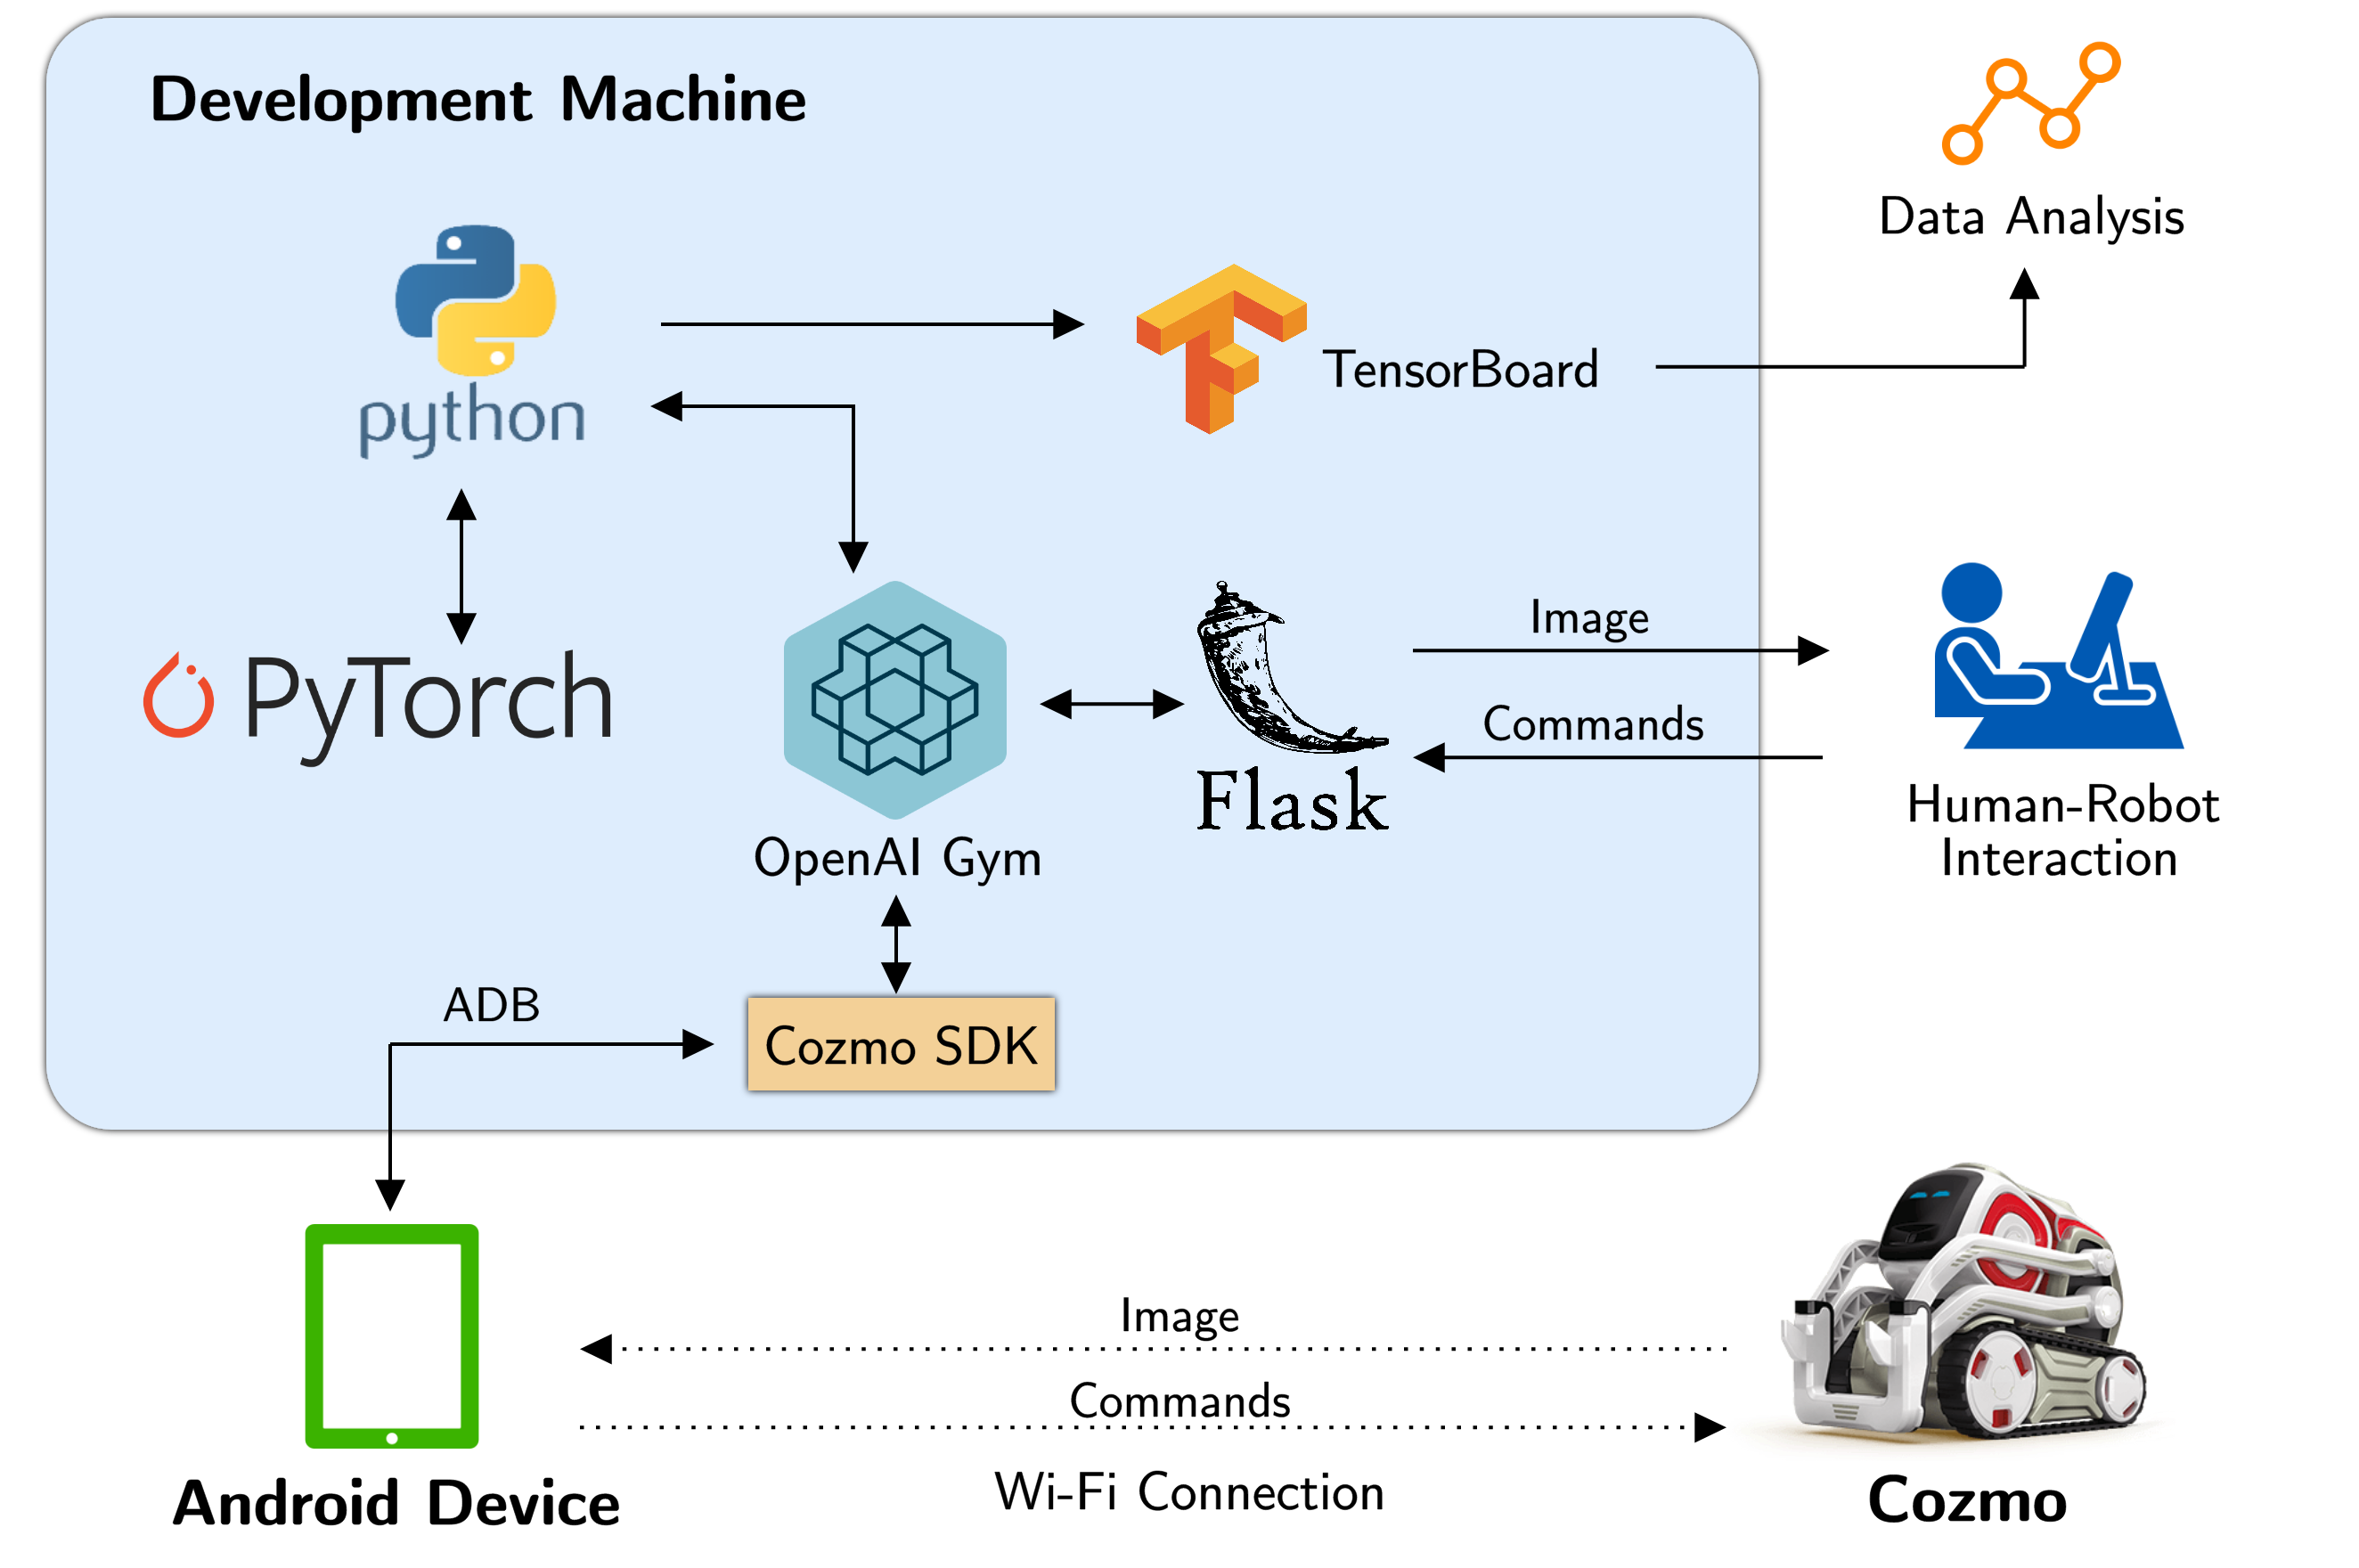
\includegraphics[width=\textwidth]{img/cozmo-system.png}
    \caption[Outline of the control system]{The interaction between the user and Anki Cozmo has a crucial role in this system.
        The main Python script utilises OpenAI Gym for the reinforcement learning component and PyTorch for the deep learning one.
        The user can interact with the flow of the system through a simple web app that uses OpenAI Gym and the Cozmo SDK directly to provide information for the user (e.g.\ images, learning information) and the robot (e.g.\ commands).
        The last component consists of TensorBoard thanks to which the script can store results that can be retrieved later by the user.}
    \label{fig:system}
\end{figure}

\subsection{OpenAI Gym Cozmo environment}

Before starting the description of the system we designed to carry out reinforcement learning experiments it is necessary to outline the decisions we made about what to implement in \textit{CozmoDriver}, the OpenAI Gym environment we developed to apply, train and test reinforcement learning algorithms with Cozmo.

The path of this section will follow the steps of a typical formalisation of the Markov Decision Process (MDP), bringing out the problems encountered, the reasoning behind them and solutions proposed as they go.

\subsubsection{Markov Decision Process formalisation} \label{subsubsec:mdp_form}

Starting from the definition of MDP that we already reported in~\vref{eq:mdp}, we studied and investigated the best configuration to provide an acceptable trade-off between performance and memory consumption, capable of making the system work on the development machine we used for our experiments.
In the following paragraphs, we will analyse each MDP aspects paying particular attention to the problems we faced and the motivations behind every decision made to overcome them.

\paragraph{State/Observation space}
The environment observation is the group of information that the reinforcement learning agent can see and obtain from the interaction with the real world.
Current autonomous driving technology usually works thanks to the presence of various sensor positioned in different points of the car body as we discussed in \vref{sec:related-work}.
However, this approach is quite different from what human beings use to guide every day: the only input that the human receives is what he sees.
Taking this fact into account, in the self-driving tasks in question, we thought that the most reasonable way to obtain knowledge about the surrounding environment as similar as possible to how humans do was to exploit front camera images provided by Cozmo SDK.
However, it is essential to remember that, by definition, the state must satisfy the Markov property.
According to this definition, \textit{the state must be independent of the past given the present}.
For this reason, using a single image to describe the current state may be an oversimplification of the problem.
Even a human would not be able to determine the best action to take starting from a single frame.
That is because it is difficult to infer or determine the current direction of the car, speed or steering wheel position.
Merely adding another image can intuitively improve the human perception of the scene: as an example, the first intuition this introduction could reveal is where the car is going, allowing the user to decide more accurately about the trajectory to follow.

To verify this fact before starting the experiments with the application of the reinforcement learning algorithms to Cozmo, we firstly analysed the results of some experiments on the environment of the classic control problem of trying to keep a frictionless pendulum standing up (\textit{Pendulum-v0}).
The original version of this environment utilises angle position and trigonometric results as observation to return to the agent.
However, this environment offers to the user the access to the images provided by the OpenAI Gym \texttt{render} interface.
It represents an entirely different kind of experiment from Cozmo driving task, but they have in common the improvement in trajectory inference brought by the presence of a number of pictures higher than one.
In order to make this environment suitable for convolutional neural networks, we decided to appropriately modify it to exploit raw images as observations instead of the original information.
Therefore, we noticed that the usage of a single picture as observation led to unstable and worse results than the ones obtained by combining two subsequential images to feed the algorithm.
For this reason, we decided to use two consecutive raw images provided by Cozmo by using a queue data structure with size two.
In the code flow, the developer merely has to push the next image obtained from the robot and use the specific queue function implemented to obtain the concatenation of the last two images, only when necessary.

Therefore, we decided to reduce the original size of the input Cozmo image to 64$\times$64.
We made this decision as a trade-off between performance, learning phase duration and space available in the central memory to store the replay memory.

In conclusion, the observation provided to the agent is the concatenation of two grayscale images with dimension 64$\times$64 pixels.

\paragraph{Action Space}

Another essential part that we needed to formalise is the action space, how the agent can interact and influence the surrounding environment.
In the car scenario, the two main components of driving are the speed of the vehicle and the position of the steering wheel.
To straightforwardly formalise these two parts, we decided to use two simple real values.

We chose to define the desired speed value in a range of 0 to 1, while we opted for a range of -1 to 1 for the steering wheel position.
These limits allow the agent to manipulate simple values in the decision-making process and to facilitate the manipulation of neural network results.
At the same time, the underlying logic of the environment takes care to translate these values into a compatible format for the Cozmo SDK.
Indeed, as reported in \vref{subsec:human-robot-interaction}, the Cozmo SDK function exploited to manoeuvre the robot needs at least the speed of each tread.
\Vref{conversionCozmoDriver} reports key steps of this translation.
Therefore we decided to raise acceleration parameters by setting them equal to 4 times the velocity of each thread to reach the desired speed as fast as possible.

\begin{algorithm}[!h]
    \SetAlgoLined
    \small
    \DontPrintSemicolon
    \LinesNumbered
    \KwIn{Desired speed $s_t \in \{ x \in \mathbb{R} | 0 \le x \le 1 \}$\newline Steering wheel position $w_t \in \{ x \in \mathbb{R} | -1 \le x \le 1\} $\newline Maximum forward speed $s^{\text{forward}}_{\text{max}} = 150\text{mm/s}$\newline Maximum turning speed $s^{\text{turning}}_{\text{max}} = 100\text{mm/s}$}

    Left tread speed: $ts_{\text{left}} = s_t \cdot s^{\text{forward}}_{\text{max}} + w_t \cdot s^{\text{turning}}_{\text{max}}$\;
    Right tread speed: $ts_{\text{right}} = s_t \cdot s^{\text{forward}}_{\text{max}} - w_t \cdot s^{\text{turning}}_{\text{max}}$

    \KwOut{Left tread speed $ts_{\text{left}}$ \newline Right tread speed: $ts_{\text{right}}$}
    \caption{CozmoDriver actions conversion from virtual to real}
    \label{conversionCozmoDriver}
\end{algorithm}


\paragraph{Reward Function}

The reward function is the crucial feature to define in the formalisation of the MDP.
After a review of the available literature and the analysis of the problem, we obtained a list of ideas and concepts to model the reward function:

\begin{itemize}
    \item \textbf{Lane Distance}: this model calculates the reward of each action by calculating the distance between the car and the centre of the lane.
          The main aim is to prioritise the correct positioning of the car on the lane, crucial for driving safety.
          However, it is noticeable that this value can be easily calculated in a simulated environment, while it needs a lot of sensors and calculations to obtain a good estimation in a real-world environment.
          Beyond this problem, this approach has difficulties in scaling to varying environments where road typology and dimension is not a pre-configured constant.
          Therefore, it is a limited approach because human beings do not always drive the car in the perfect centre of the lane: for instance, when approaching a curve, it could be more convenient to move the car slightly away from the perfect centre.

          This fact reveals the shortcomings of this approach: the system can perform only as good as the human intuition underlying the hand-crafted lane reward.

    \item \textbf{Distance Covered}: the second approach we investigated was the one suggested by~\cite{kendall2018learning,kendall2019learning}, where the reward of a specific action consists of the total distance covered by the car for each specific action taken.
          Approaching the problems with this method leads to results that can be easily understandable for humans: indeed, the total reward of each episode represents the total distance travelled by the robot.

          In the car scenario of the previously mentioned publication, it is possible to use the car odometry device to quickly retrieve this value after each action and calculate the reward of a specific decision obtaining the difference with the previous value.
          Cozmo does not have such kind of sensor on board.
          Therefore it is necessary to calculate this value manually.
          The intuition behind a reasonable estimation of the distance covered by Cozmo consists of using the fundamental formula of kinematics: the speed.
          Indeed, in the designed system, we have direct access to the aspired speed because it is a parameter that the agents decide at each iteration, and it is possible to derive the time elapsed between one action and its following one by manually calculating them inside the OpenAI Gym environment.

    \item \textbf{Speed Crash Penalty}: the third typology of reward we investigated consists of a sort of life bonus reward.
          The robot receives a reward (e.g.\ 1 point) for each timestep of correct decisions and a negative reward (e.g.\ -10 points) every time the user stops the robot preventing the crash.
          Therefore we added to the positive reward a small quantity that depends on the current speed to encourage the robot to stay on track and increase its speed.
          Consequently, we decided to add a penalty in faulty time step proportional to the robot crash speed to entice the robot in avoiding high speed when close to critical points.
          \Vref{eq:speedCrashPenalty} formalises the reward used in this approach: $p_1$ and $p_2$ are two parameters that determine how much the speed influence the reward and their module must be much less than the constant value in the equation to highlight the fact that they represent a secondary objective \cite{raffin2019learning}.
          \begin{equation}
              r_t = \begin{cases}
                  +1 + p_1 \cdot s_t, & \mbox{if } \mbox{Cozmo on the track} \\ -10 - p_2 \cdot s_t, & \mbox{if } \mbox{Cozmo off the track}
              \end{cases}
              \label{eq:speedCrashPenalty}
          \end{equation}

\end{itemize}

After the analysis of these three reward design proposal, we decided to select the second one to pursue our experiments in the real world.
As previously reported, the first option would have been hard to carry on and to scale up.
The third option hints intriguing facts that a reinforcement learning agent could take into account to better solve the driving task of our experiments.
The only withdrawal of this approach is related to the correlation between reward and distance covered: this correspondence is significant for the developer to have a more transparent overview of what is happening and how the algorithm is learning, at least in the early stages of development.
In the second option, the distance covered by the robot is equal to the reward, while this conformity is lacking in the third option.
For this reason, we decided to take the second reward proposal for this time.
We noticed that it could be an exciting future development trying to merge the second alternative with the third one to obtain a brand new reward function that both penalises bad decisions proportionally to speed and maintain its correspondence with the track crossed.

\subsection{Human-Robot interaction} \label{subsec:human-robot-interaction}

\begin{figure}

    \centering
    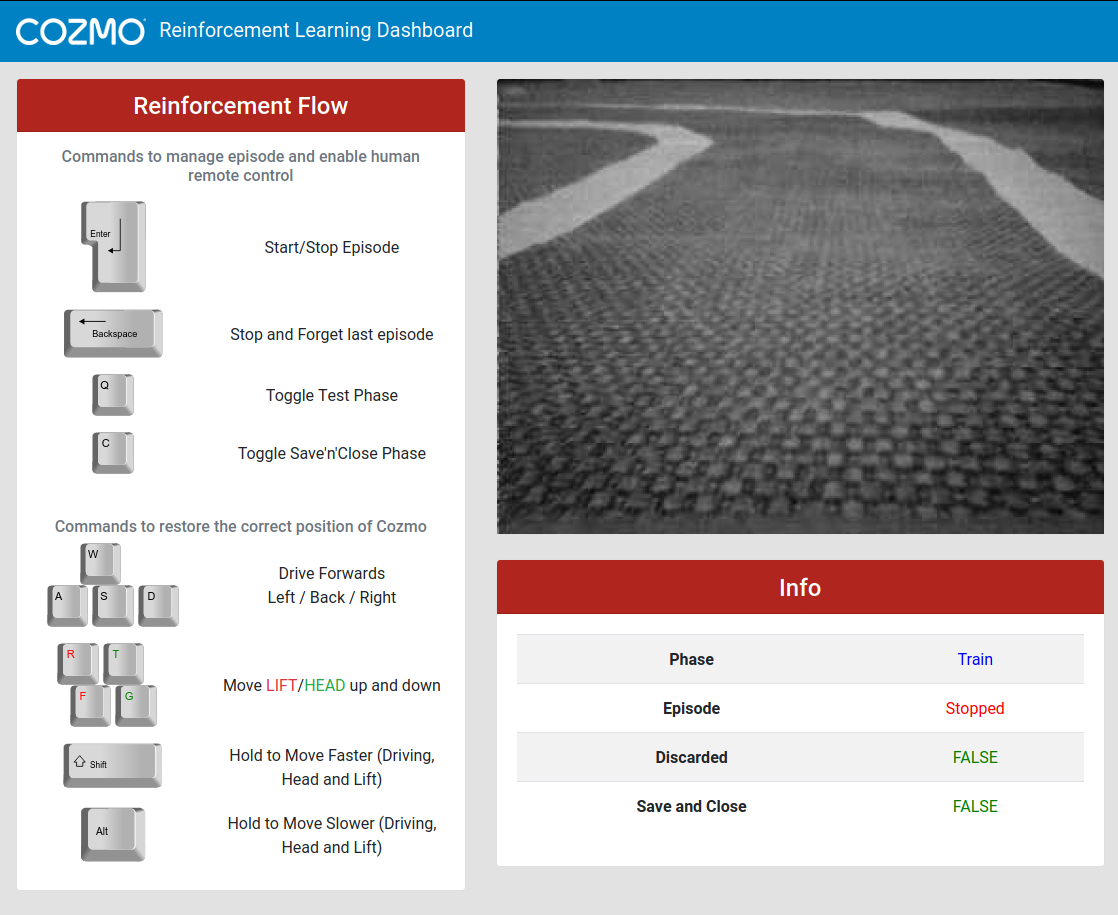
\includegraphics[width=\textwidth]{img/dashboard.png}
    \caption[Web Application implemented to Control Cozmo]{This image shows the web application we implemented to control Cozmo during reinforcement learning experiments.
        The focus is on the first two columns of the application since they provide the essential tools.
        The first one is entirely dedicated to the list of key the user can use to drive the robot or control the reinforcement learning algorithm flow.
        The second column consists of the live image coming from Cozmo front camera and some information about the current state of the RL system.}
    \label{fig:dashboard}
\end{figure}

It is noticeable that the simulator can undoubtedly be programmed to understand whenever the car is going outside the track, crossing the roadside.
In a reinforcement learning scenario, this fact facilitates the restarting procedure for an episode: the developer has to bind some events or actions to a process that stops the current episode, put the car on the road again and starts the next experiment.
In the real world, the situation is more complicated not only because of the need of the human intervention to relocate the car in a safe place but also because there are more variables to take into account.
The most critical factor is that the failure of an episode in the simulator has no threats or costs, while real-world experiments failures could lead to high costs and severe damage to the car and equipment.
Despite this point, the application of such experiment typology in a real environment instead of a mere simulation represents an exciting challenge that could bring reinforcement learning to the next level.
In order to make experiments as safe as possible, the authors of~\cite{kendall2018learning,kendall2019learning} implemented a self-driving system designed explicitly for self-driving reinforcement learning experiments where the car driver has the faculty of stopping the car when it is going to run off the road or in a dangerous situation and relocating it in the nearest safe position to start the next learning episode.
By simply pressing a button, the logic of the car disables reinforcement learning algorithm decisions and gives full control to the real driver of the car.

We aimed to implement this kind of user-robot interaction also in our setup.
The requirements were almost the same as the ones described in the paper, but this case could not rely on steering wheel, brakes and accelerator as in the car scenario where they are directly accessible by the user.
The system needed an interface to allow the developer to stop the robot whenever it is approaching the side of the road and manoeuvre the robot just like a car.
For this reason, we firstly implemented a straightforward interface using a web app implemented using plain HTML5, CSS3 and Javascript for the frontend and Flask \footnote{Flask Github Repository: \href{https://github.com/pallets/flask}{https://github.com/pallets/flask}}, a lightweight Web Server Gateway Interface (WSGI) web application framework, as backend.
Therefore, we designed the web-app interface by using the Bootstrap framework \footnote{Bootstrap documentation: \href{https://getbootstrap.com/}{https://getbootstrap.com/}} to offer an easy-understandable and appealing user experience.
A screenshot of the dashboard is available in \vref{fig:dashboard}.

The aim of this application is allowing user interaction with Cozmo and Flask represented the right choice to allow the communication between this interface and the OpenAI Gym environment.
The Flask backend interacts directly with the functions offered by Cozmo SDK to allow the user to see the live streaming from Cozmo camera directly in the web app.
Therefore it can receive, convert and forward commands from the robot to the SDK.
These commands consist of the pressure of both single or combination of buttons: Flask decides the action to trigger programmatically with hard-coded conditions and calculates speeds and accelerations of both right and left treads.

The SDK function we utilised to control Cozmo is \texttt{drive\_wheels()}.
The parameters of this function are the following:

\begin{itemize}
    \item \textbf{\texttt{l\_wheel\_speed}} (\textit{float}): mandatory parameter that specifies the speed of the left tread (in millimeters per second).
    \item \textbf{\texttt{r\_wheel\_speed}} (\textit{float}): mandatory parameter that specifies the speed of the right tread (in millimeters per second).
    \item \textbf{\texttt{l\_wheel\_acc}} (\textit{float}): optional parameter that specifies the acceleration of the left tread (in millimeters per second squared).
          The default value is the equal to \texttt{l\_wheel\_speed}.
    \item \textbf{\texttt{r\_wheel\_acc}} (\textit{float}): optional parameter that specifies the acceleration of the right tread (in millimeters per second squared).
          The default value is the equal to \texttt{r\_wheel\_speed}.
    \item \textbf{\texttt{duration}} (\textit{float}): it specifies the duration of the driving action of the robot.
          It calls \texttt{stop\_all\_motors()} after this duration has passed.
          The default value is \texttt{None}.
          In this case, the behaviour of this function is equivalent to the non-async \texttt{drive\_wheel\_motors()} one: the wheels will continue to move at that speed until commanded to drive at a new speed.
\end{itemize}

This method is the same we used to implement the OpenAI Gym environment, allowing the algorithm to interact with the robot just like a human in the driving seat.
Just as examples, the user can start and stop the episode using the enter button, forget the previous episode with backspace and relocate the robot on the track using W, A, S and D buttons.

\subsection{System flow} \label{subsec:system-flow}

The implementation of an algorithm flow to sustain the specific experimental need was necessary due to the continuous interactions between the human and the robot.
Starting from the ideas of \cite{kendall2018learning,kendall2019learning}, we decided to divide the learning process in a series of phases highlighted in blue in \vref{fig:system-flow-chart}.

\begin{figure}
    \centering
    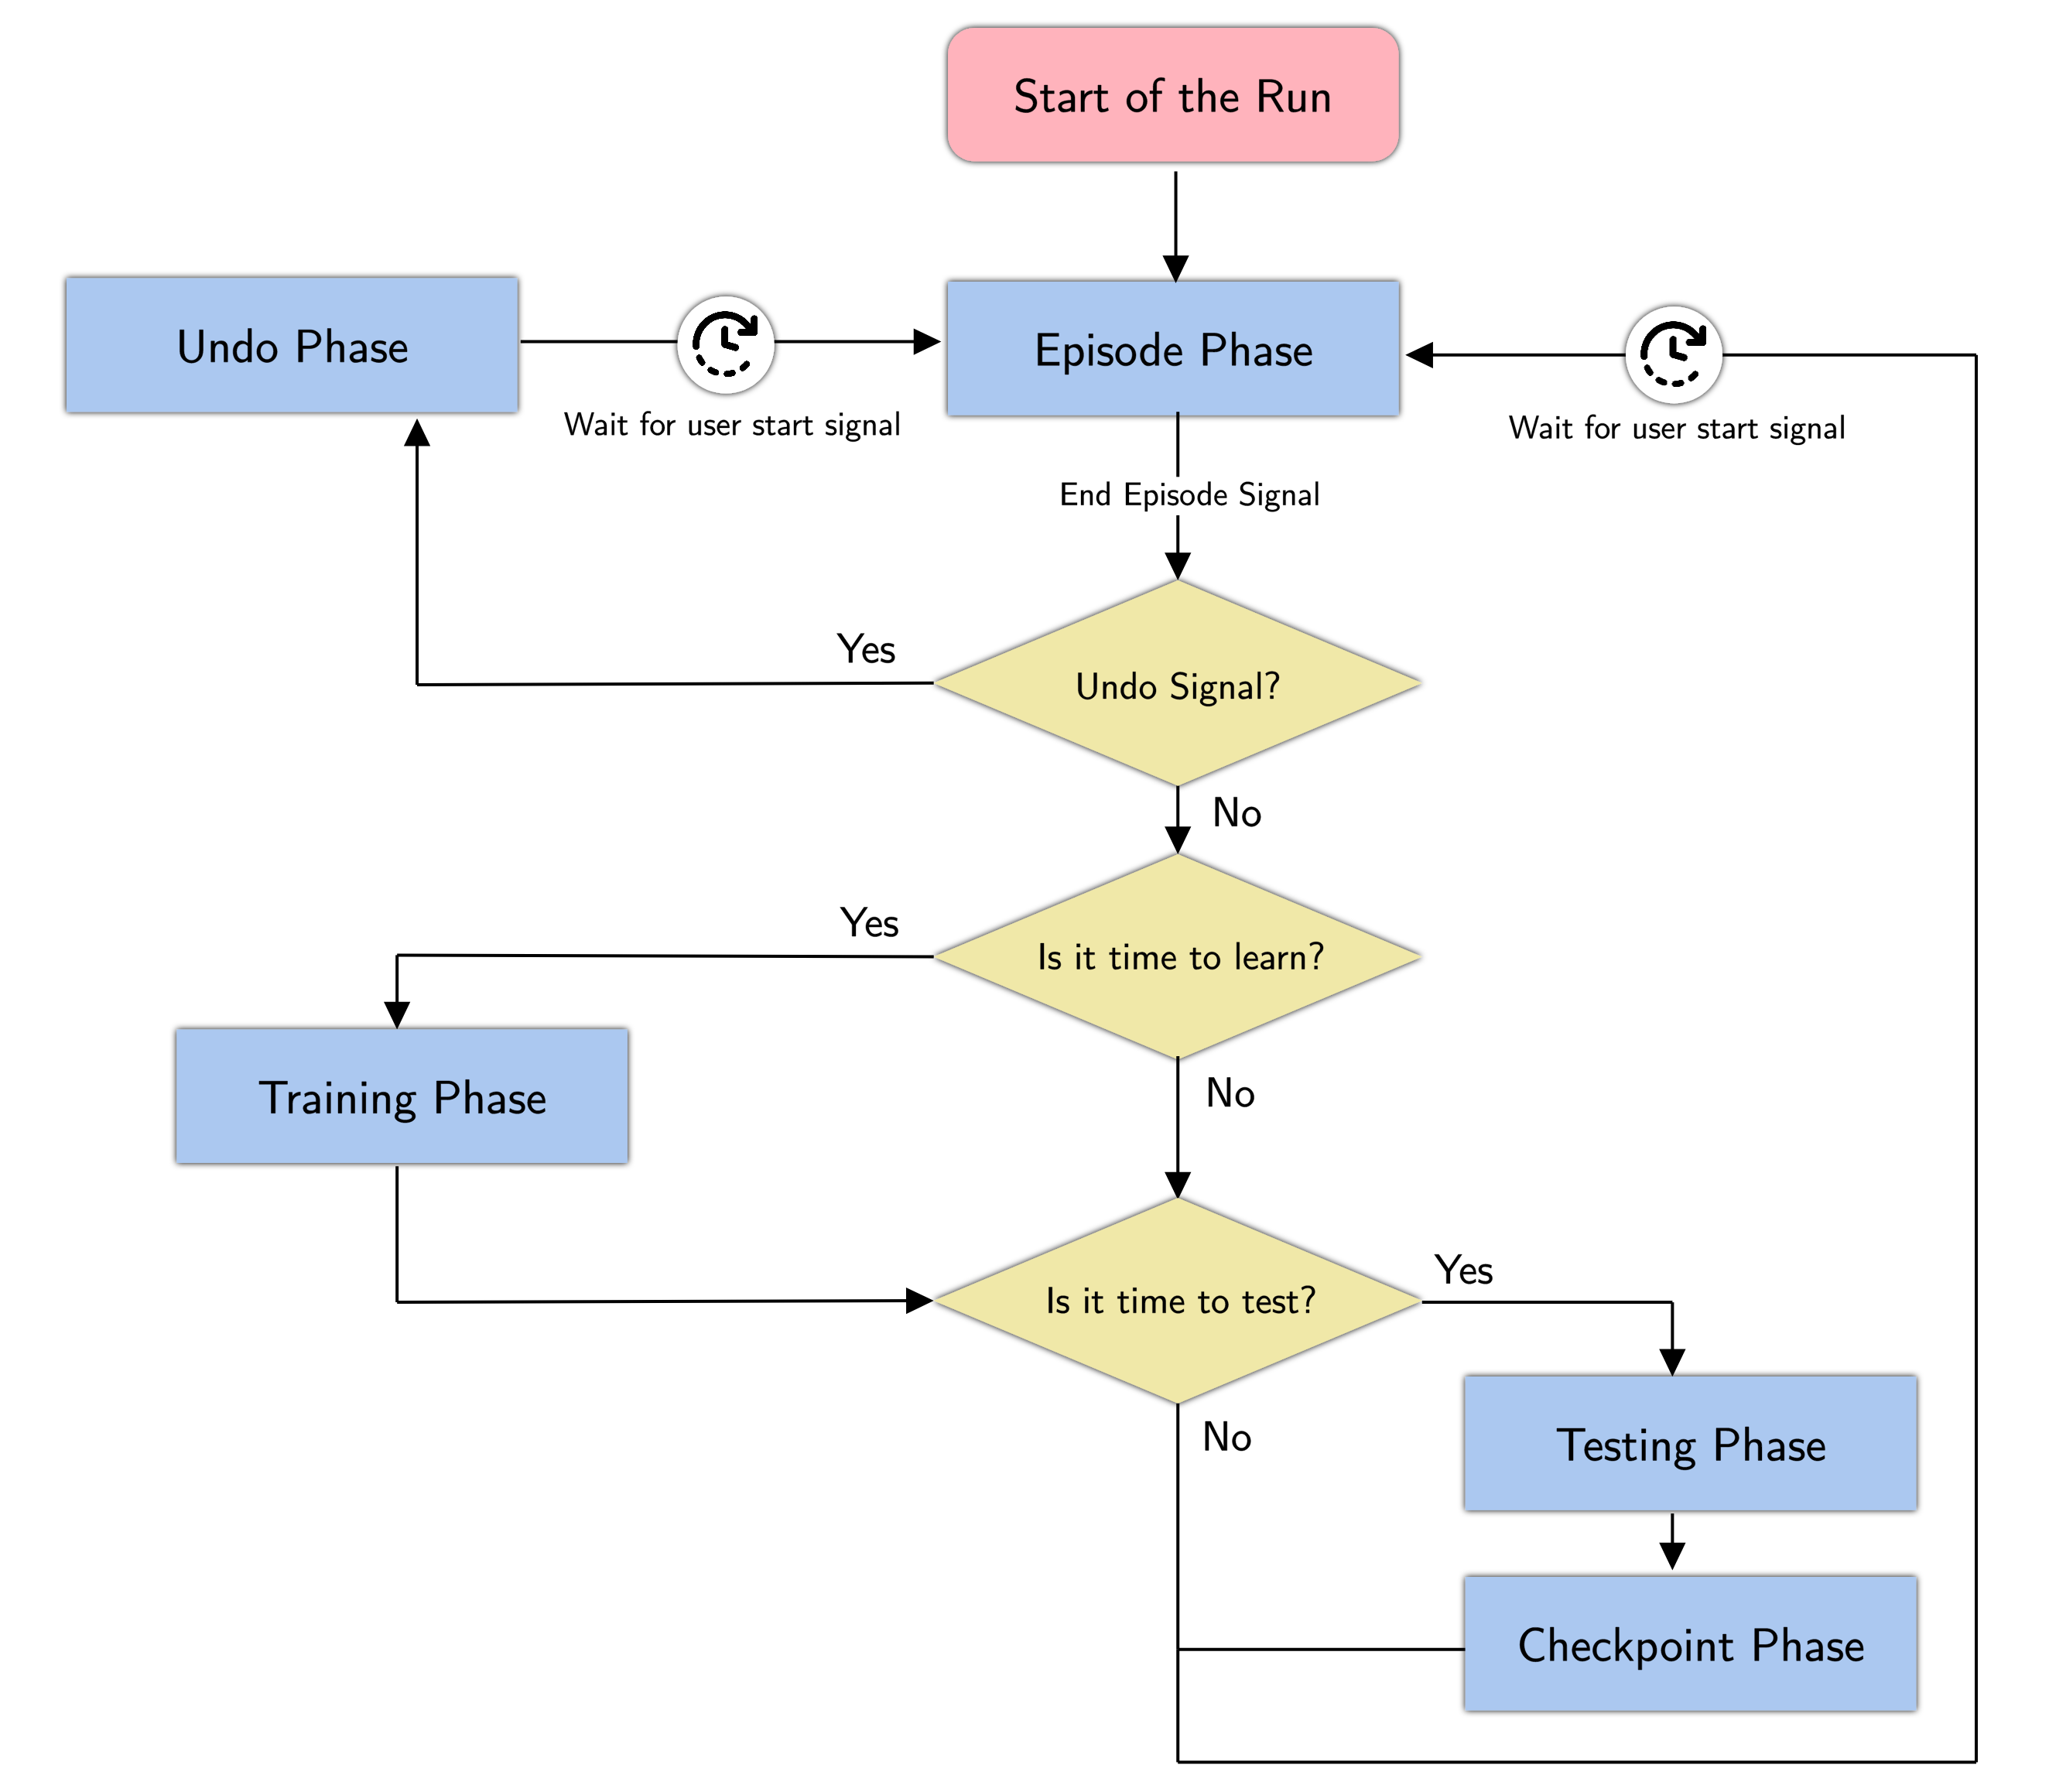
\includegraphics[width=\textwidth]{img/system-flow.png}
    \caption[Cozmo algorithm flow chart]{This image shows the flow chart of the system we implemented.
        The most crucial phases are highlighted in blue.
        This chart is deliberately drawn without an end, because, although there was the possibility, we never set a fixed maximum limit of experiments in Cozmo scenario.
        It is possible to retrieve the warm-up procedure by answering no to the last two decision branch.}
    \label{fig:system-flow-chart}
\end{figure}

The phases we defined are the following:

\begin{itemize}
    \item \textbf{Episode phase.} This phase consists of a single episode take.
          It represents the results of a series of action taken from the agent to solve the task.
          In the early part of the experiment, the algorithm has to perform a warm-up, a procedure where the agent makes random actions to explore the environment randomly and obtains an initial set of entries for experience replay memory.
          After the agent gathered the minimum amount of entries, which is usually equal to the batch size or a multiple thereof, the agent starts to exploit the neural network to act using a noisy policy for exploration purpose.
          This last-mentioned part is still an episode phase, but testing or checkpoint phase never follows it.
          As reported in \vref{subsec:actions-duration}, the time between two subsequent actions is a parameter we set according to limitations of Cozmo SDK to avoid problems in the learning process.

          The user is the main responsible for this phase.
          It can interact by toggling enter button on the keyboard.
          The first hit starts the episode, while the second one determines the end of the episode and attributes zero rewards to the last action taken.

    \item \textbf{Undo phase.} As described in \vref{subsec:error-management}, it is possible to invalidate experiments due to a human or a system error.
          For this reason, we implemented a procedure that the user can trigger to delete the knowledge acquired in the last training episode and restore the previous state.
          We positioned it right after the episode phase to delete faulty episodes as soon as possible.

          In this case, the user has two possibilities to undo the last episode.
          The user can either hit the backspace button in substitution of the second enter button hit to stop the episode and start the undo phase or pressing it after the end of the episode and before the next one.
          Initially, the first choice led to a direct restore of the previous situation without executing the training phase, while the second one executed the training phase and only afterwards the undo phase.
          After some tests, we decided to set the first behaviour as unique for both possibilities.
          This choice led to a delay increase between two consecutive episodes because of the addition of an indirect confirmation of the current episode before starting the training phase. However, thanks to the careful design of the network, the waiting time remained manageable.
    \item \textbf{Training phase.} This section starts its execution after the initial warm-up phase, and it is located after each Cozmo episode.
          It manages all neural networks updates with several optimisation steps, also known as epochs: the number of optimisation steps is set as a parameter by the developer.
    \item \textbf{Testing phase.} This phase disables noisy policies from the algorithm to allow the agent to take the action that the neural network decree as best in that specific iteration.
          It consists of a repetition of a finite set of episodes that triggers after every specified number of epochs, given as parameter of the system: the average reward calculated by the rewards obtained from each testing episode is the result of this phase.
          This value is crucial for the reinforcement learning experiments because we used them to build the average reward performance graph that shows how much the agent learned in the graphs of \vref{ch:ch5} and determines the quality of the learning process itself.
    \item \textbf{Checkpoint phase.} This phase is described in \vref{subsec:error-management}.
          It consists of saving all data to make the developer able to restart the experiment from the last available checkpoint.
          It is usually located right after the testing phase in order to save all values together with network weights and biases.

          The user can also trigger this phase manually by toggling the C button before starting the next episode by hitting the enter button.
          It allows to virtually pause experiments, like the one with Cozmo, that could last tens of hours, and that can need multiple days to complete.
\end{itemize}



\section{Algorithm setup}

% TODO: DDPG-SAC?
Another crucial step in the design of the system is the setup of reinforcement learning algorithms we exploited.
This thesis aims to show results and challenges of the implementation of SAC algorithm to solve a real-world driving task, so it is essential to include in this document ideas and implemented choices we used to develop our system.

Given the fervour that has led to an impressive development of reinforcement learning in recent years, numerous repositories were born to be able to offer ready-made implementations of these algorithms in order to speed up the implementation process in the most suitable experiments.
Nowadays, the most famous and exploited reinforcement learning repository available for developers is \textit{OpenAI Baselines} \footnote{OpenAI Baselines Github Repository: \href{https://github.com/openai/baselines}{https://github.com/openai/baselines}} which provides a set of high-quality implementations of reinforcement learning algorithms realised using \textit{Tensorflow} deep learning library.
In addition to this last-mentioned project, there are many new forks of this project which offers improvements, refactorings or additional implementations of the latest algorithms offered by the continuous scientific research in this field.

Despite this fact, we decided to implement our versions of reinforcement learning algorithms from scratch taking the last-mentioned implementations as guidelines to follow in the developing process instead of exploiting them directly.
We chose to follow this workflow primarily for didactical reasons.
Implementing an algorithm from scratch, starting from the theory provided by the related paper escorted by the numerous implementations available is probably the best way to understand the whole set of ideas underlying algorithms properly.
Furthermore, we made this decision to have the opportunity to manage and implement architectural choices to create a suitable workflow for the episodes carried out in Cozmo experiments that could be compatible with the human-robot interaction of Cozmo.

This section contains the choices we made in the design of the neural network and a reflection about the selections made for the hyper-parameters of reinforcement learning algorithms.

\subsection{Neural networks design}

Another essential component in the developing of the control system is the convolutional neural network we designed.
As already reported in chapter 3, we opted using PyTorch as deep learning framework.
To choose the neural network that could better meet the requirements, we analysed the models used in~\cite{lillicrap2015continuous,kendall2018learning,haarnoja2018soft, haarnoja2018alg}.

The author in~\cite{lillicrap2015continuous} presented two types of neural networks, but the model we are interested in is the convolutional one, used to learn from pixels.
It consists of 3 convolutional layers without pooling with 32 filters at each layer.
Therefore, the authors added two fully connected layers with 200 units.
The paper also contains information about the initialisation of network weights and biases: they set final layer ones from a uniform distribution of $[-3\times 10^{-3},3\times 10^{-3}]$ and $[-3\times 10^{-4},3\times 10^{-4}]$ respectively in order to ensure the initial outputs for the policy and value estimates were near zero.
They used uniform distributions $[\frac{-1}{f^{0.5}}, \frac{1}{f^{0.5}}]$ where $f$ is the layer fan-in.
The actions were concatenated just before fully connected layers.

In \cite{kendall2018learning}, the authors used a convolutional neural network with four convolutional layers, with 3$\times$3 kernels, a stride of 2 and 16 feature dimensions, shared between the actor and critic models.
Therefore, the flattened encoded state obtained from convolutional operations were used as input for fully connected layers of both actor and critic: in the last case, it was concatenated with the actions.
In this architecture, there was only a single fully-connected layer of 8 features.
They conducted the experiments using a modified Renault Twizy vehicle with a single forward-facing video camera situated in the centre of the roof at the front of the car, carrying out their experiments on-board using a single NVIDIA Drive PX2.
They managed to solve their self-driving task in a handful of trials using 250 optimisation steps with a batch size of 64.
They managed to make the experiment very manageable with an optimisation phase that took approximatively 25 seconds, which is a reasonable amount of time considering that the driver must reposition the car at the centre of the lane before restarting the procedure.
As stated in the paper, their agent was able to cover a distance of about 300 metres in 37 minutes of training time within just 35 episodes.
In the real world, the environment is much more complicated than the simulated one, and then they decided to implement the logic of the agent through the usage of a Variational Autoencoder (VAE).
This decision led to an improvement in the reliability of the algorithm.

In \cite{haarnoja2018alg}, the authors reported the training of a real-world robotic task with a 3-finger dexterous robotic hand.
The objective of the agent is to position a sink faucet in a specific position highlighted by a coloured end.
The neural network exploited on this occasion consisted of two convolutional layers with 3$\times$3 filters and max-pool layers, four features and followed by two fully connected layers with 256 units.
Even in this case, the authors exploited RGB images to carry out real-world training of the agent.
Therefore, they included some information about training time: the agent needed 300k environment interaction steps with an equivalent of 20 hours of training.

The problems just outlined have relative differences, but the varying durations of the experiments are truly impressive.
This fact underlines how the training duration depends not only on the data quality but also on hyper-parameters used, on the complexity of the problem and the available computational power.
It is the primary motivation behind the elaborateness of an experiment carried out entirely in the real-world.

After the analysis of the neural network used in the last-mentioned papers, we tried to modify these models after testing them on a modified version of the \textit{Pendulum-v0} environment, provided by the OpenAI Gym framework, with a variety of architectures.
We exploited the network architectures that passed this selection to made experiments with \textit{Pendulum-v0} and, consequently, with the environment we designed with Cozmo.
\Vref{ch:ch5} will show the results in question.

However, before finding a good architecture to exploit, we started little experiments with Cozmo to analyse changes in the behaviour policy of the robot.
There we noticed a crucial factor to take into account to decide what network to use for our experiment: the optimisation phase duration.
It is a vital parameter to make the experiment manageable for the user: in this thesis work, the agent is not in a simulation where the computer automatically decides when to restart the episode so that the human can let the experiment running by itself.
In this context, the user must be ready to stop, reposition and restart the car at any moment.
Given the evidence that an experiment like this could last thousands of episodes, we aimed to reduce the waiting time for the user to make the experiments last less, or, at least, obtain a good relationship between the duration of the episode and that of the optimisation steps.
To avoid a long waiting time after each episode, we tried to spread the optimisation phase inserting a single learning step after each action taken by the agent.
We found out this approach in some implementation of DDPG algorithm mainly applied to simulated environments.
This choice seemed working with the \textit{Pendulum-v0} task because, in a simulated context, the environment stops itself waiting for the next action taken by the agent during the optimisation phase: the system flow is independent of the duration of the last-mentioned phase.
It is noticeable that this fact does not apply to a real-world scenario like the one we implemented with Cozmo.
As discussed in \vref{subsec:actions-duration}, the robot continues to drive even during the learning process.
Therefore the system is highly unstable because this process not always has the same length and every action lasts differently: it depends on the specific network topology.
After the analysis of this behaviour, we decided to maintain the optimisation phase among episodes and to fix a specific duration for each action of Cozmo.

The architecture we selected was a sort of merge of the ones we found in \cite{kendall2018learning,kendall2019learning,haarnoja2018alg}.
We opted for a neural network with three convolutional layers with 16 features of 3$\times$3 dimension.
We decided to use a stride of 2 instead of using pooling layers with a stride of 1, following ideas of the authors of \cite{kendall2018learning,kendall2019learning}.
This decision aims to shorten the optimisation phase and obtain more manageable experiments without impacting performance excessively \cite{springenberg2014striving}.
We applied batch normalisation after each convolutional level to improve the speed, performance, and stability of neural networks \cite{ioffe2015batch}.
Finally, we flattened the results and used them as input for the last part of the architecture, which consists of two fully-connected layers with a hidden size of 256 features.
We decided to implement the network using the Rectified Linear Unit function (ReLU) as non-linearity, to initialise all network biases to 0 and all weights using Xavier initialisation \cite{glorot2010understanding}.

In the Q-Network implementation, the outputs of the convolutional section were concatenated with actions, and there is one single output value after the fully-connected part, which represents the value of the action-value function $Q$.
In the policy scenario, as shown in \vref{fig:cnn_cozmo}, there is no concatenation at the end of the convolutional layers stack, and the output size depends on the dimensionality of the specific action space which, in the Cozmo scenario, is equal to 2.

\begin{figure}

    \centering
    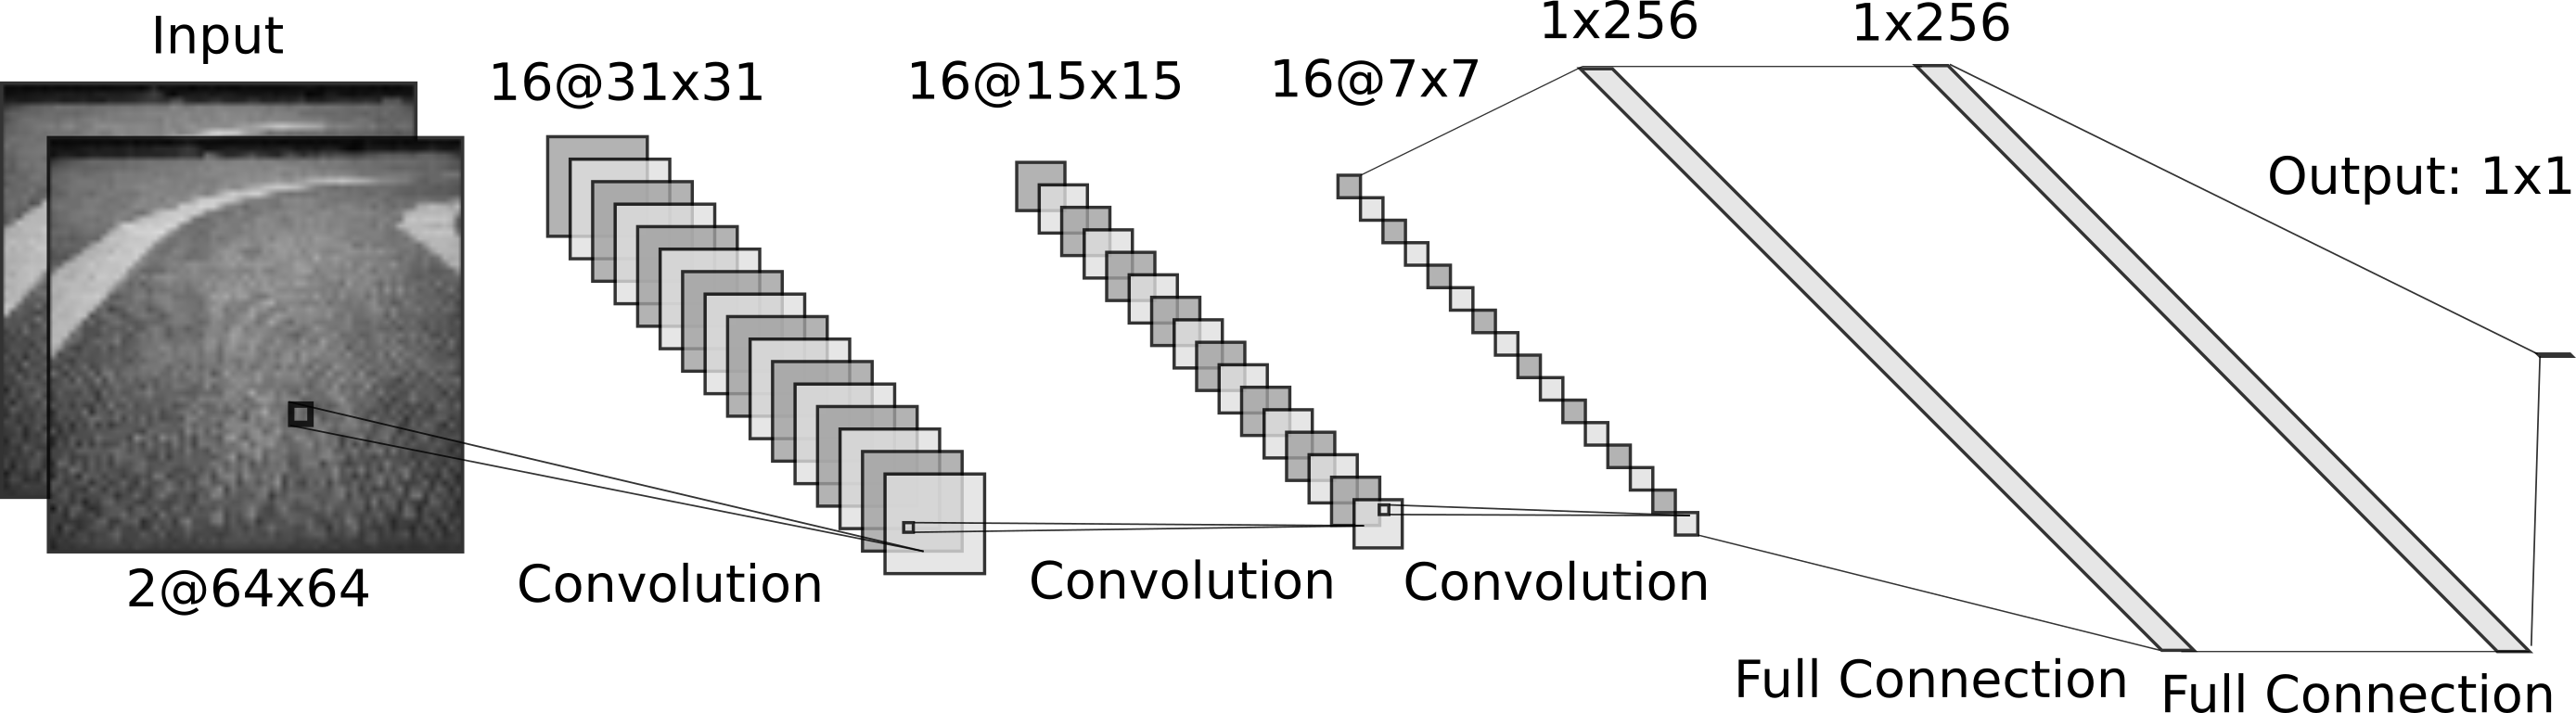
\includegraphics[width=\textwidth]{img/cnn_cozmo.png}
    \caption[Convolutional Neural Network Architecture for Cozmo experiments]{ Convolutional Neural Network Architecture for Cozmo experiments.
        This particular example shows the model exploited as the Policy with a tensor with dimension equal to the action space size as output and two consecutive grayscale images which represents the state of the environment as input.
        The first part of the network consists of three convolutional layers with 16 features of 3$\times$3 dimensions.
        Each level is supplemented by a batch normalisation one.
        The results are then flattened and concatenated with the vector of actions before entering the second part.
        This section consists of two fully-connected layers with 256 features.
        The output of this particular network represent the action to take, given the input state.
        This network uses ReLu as non-linearity.
        Before starting experiments, the network is initialised with biases equal to zero and weights set utilising Xavier initialisation \cite{glorot2010understanding}.}
    \label{fig:cnn_cozmo}
\end{figure}

\subsection{Algorithms implementations and hyperparameters}

As already mentioned in this section, the experiments we made in this thesis were carried out in a real-world environment.
At the beginning of this thesis work, we implemented the DDPG algorithm following the theory of the related paper and the hyperparameters suggested in \cite{lillicrap2015continuous,kendall2018learning,kendall2019learning}.
This process was carried out in parallel with the implementation of the same algorithms for a simulated environment offered by the OpenAI Gym framework, \textit{Pendulum-v0}.
This decision was useful to check the correctness of the architectural decisions we made step by step.
Despite this fact, the learning context of Cozmo showed its complexity since the first experiments bringing out differences from \textit{Pendulum-v0} environment.
We found out that, in order to obtain results that could show as clearly as possible whether the algorithm is working and improving with the selected set of parameters, it was necessary to wait for a large number of epochs corresponding to tens of hours or few days depending on the neural network architecture and the hyper-parameters.

% TODO: DDPG SAC ?
Furthermore, these experiments can not exploit the advantages of the simulated environment in which the researcher can set the parameter ranges at the beginning, leaving the computer to start and complete the search for each combination of the available parameters.
The real-world approach we described in this chapter needs the constant presence of a human to carry out the learning process, and the whole procedure is further slowed down by the Cozmo battery lifetime and its charging time: both take about 30 minutes.
It is noticeable that, in a real-world scenario like this, it is almost impossible to make a humanly manageable workflow capable of doing a sustainable grid search.
For this reason, we decided to initialise these parameters following the guidelines provided by the DDPG paper.
The results, in this case, were not as good as we expected: the robot showed no tangible progress even after numerous episodes.
The policy learned led to strange behaviour with sharp turns in a direction and episodes that ended almost immediately.

% TODO: DDPG SAC ?
After this implementation, we started a search for a reinforcement learning algorithm more suitable for real-world problems.
The ideal objective would be to find a hyperparameter agnostic algorithm capable of performing well regardless of algorithm configuration and ensuring the absence of unfairness introduced from external sources \cite{henderson2018deep}.
The last-mentioned aim is still being researched today by the scientific community.
Despite this fact, we found out an algorithm capable of automatically adapt itself to reduce the hyper-parameter dependency: SAC, an algorithm which was born precisely as an evolution of the DDPG approach to improve its performance in real-world applications and overcome hyper-parameters dependencies.
Therefore, we also implemented this algorithm from scratch by using the implementation of the so-called \textit{parameter auto-tuning} proposed in \cite{haarnoja2018soft, haarnoja2018alg}.
\Vref{ch:ch5,ch:ch6} will present the performance comparison between these two algorithms in a \textit{Pendulum-v0} simulated environment and the performance of SAC in the real-world Cozmo one.

\section{Real-World experiments}

The real-world nature of the approach we followed in the work of this thesis revealed more questions and problem than the corresponding simulated environment.
This fact happens because executing a self-driving task in the real world is meaningfully more challenging.
There are plenty of factors that inevitably emerge, and that can not be monitored and audited appropriately if not after making a large number of attempts.

This section aims to describe the most crucial and interesting problems we faced in the development of this control system together with a debate on possible countermeasures.

\subsection{Actions duration} \label{subsec:actions-duration}

In the first implementation of the environment, the agent was able to make decisions without a specific timing between actions.
This fact led to different problems in the implementation of reinforcement learning agents.
The first problem was related to experience memory gathering also caused by the limitation of Cozmo Camera: it is a 30fps camera but, as reported in the documentation of Cozmo SDK, the Cozmo framework emits a new camera image generally up to 15 times per second.
Therefore, the frequency of image requests was very high because the system did not contain timing implementation constraints in the control of operations.
These two factors led the system to retrieve the same image both before and after taking the current action.

Consequently, the state of each environment step consisted of the concatenation of two images that were often the same picture.
This consequence led to a conceptual error that may influence the process of learning if we observe that with a human perspective: a state of this kind represents an action that does not impact the environment of the system while it is modifying it.

We noticed this problem because, in the first part of the experiments, where the agent takes random action to explore the surrounding environment, the robot continued to drive a straight path, even if shaky, without taking a definite step in a specific direction and with an almost constant speed.
This symptom was strictly related to the robot's inability to have the right time to carry out a specific action before interacting with the environment with the next one.
Accordingly, the robot ends up navigating with an average speed close to the half of the maximum speed and always going in a straight line only with small and temporary slopes to the right or left.
After noting this problem, we fixed it by hard-coding a minimum interval between the execution of a specific action and the beginning of the next one in the OpenAI Gym environment: we selected this value according to the constraint given by the Cozmo SDK about robot camera device.

\subsection{Driving bias}

As we reported in \vref{subsec:human-robot-interaction}, the user has to interact with the robot to indicate how valuable is the last action taken by the robot agent.
It is noticeable that, in this context, human-robot interaction has a crucial role in the learning process.
As the sole source of information for the algorithm, it is responsible for all improvements and imperfections of learning process results: the robot learns which actions are valuable and which are unprofitable or disadvantageous, but it is essential to remember that the human is the one who decides the correctness of each action by stopping the car in a dangerous situation.
This fact inevitably leads to the introduction of unconscious bias in the algorithm that could affect final results.

It emerged after many episodes, where the robot started to learn how to steer near a curve: sometimes the robot managed to make the curve correctly, without going out of the road line, other times it was able to steer with a tread slightly out of the track, then continuing to drive correctly in the next straight section.
Since the reinforcement learning agent uses the reward received and the stack of images that represent the previous and next state in order to understand the value of a given action, the algorithm considers the last-mentioned approaches to the curve equally valuable.
From a human perspective, imperfectly executing a curve can still be considered correct, but the risk is that experiences of this type may influence the experience replay memory and then the learning process in the long term.
This factor is accentuated by the fact that, as the algorithm improves, borderline cases of this type tend to increase more and more, and the user is more and more inclined to accept them.

However subjective the error may be, we have always tried in our experiments to be as severe as possible in accepting episodes to the limit of acceptability.
We will discuss the experiments and their results thoroughly in \vref{ch:ch5,ch:ch6}.

\subsection{Error management} \label{subsec:error-management}

Despite the care taken in the design of the reinforcement learning system covered by this chapter, many factors sometimes invalidated the experiments launched.
Just to cite a few of them as an example, we can report the instability in the Cozmo connection with its SDK caused by cable failure or the discharge of the robot battery in the middle of an experiment without any warning signal.

These events can also be added to those caused directly by the distraction of the user who guides the learning process: sometimes it happened that the user sent the episode end signal when the error was already made and over.
The agent had already started to insert wrong and off-road experiences in the replay memory, invalidating the experiment carried out up to that moment.

To try to solve the problem, we have implemented two types of rescue systems.
The first is a volatile backup system for every single episode that is discarded after the start of the next one.
Once the episode has ended, if the user believes that it has not been carried out correctly or a factor has occurred that risks compromising the entire learning process, there is the possibility to restore the previous state of the episode and start the process again from that point.

We implemented the second type of rescue as soon as the experiments proved to last longer than expected.
Because the experiments could take many hours or even days, it was necessary to implement a checkpoint system to save the state of the experiment and to restore it in the following days.
We decided to insert this process at the end of the periodic test phase: it serialises and stores in the secondary memory storage the values of the neural network and the data of the reinforcement learning algorithm.

\subsection{Track design}

In order to carry out real-world experiments with Cozmo, we need to build a track specifically designed for robot dimensions.
For this reason, we spent some time to search for the most reliable way to build a path where to train Cozmo efficiently.

\begin{figure}
    \centering
    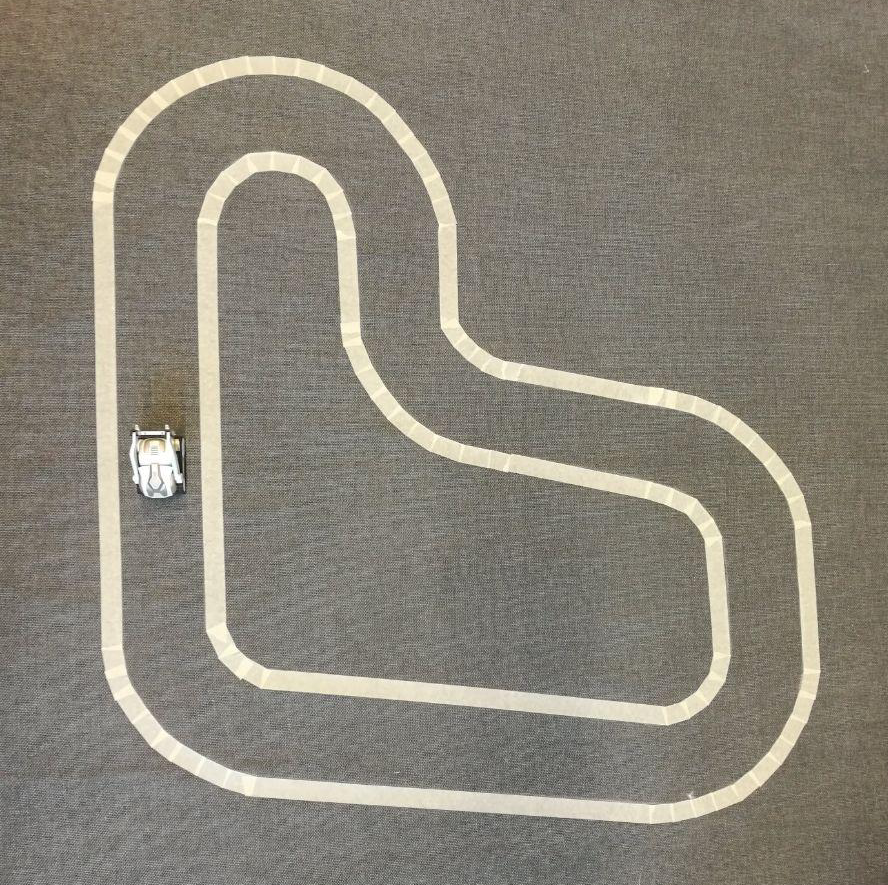
\includegraphics[width=0.64\textwidth]{img/track.png}
    \caption[CozmoDriver Racing Track]{ Picture from above of the track we designed and build to carry out experiments with Anki Cozmo robot.
        The route is a mixed track that includes two straights, a narrow hairpin and a wide one that, united by a curve elbow, make up a serpentine.
        The track length is about 3 metres.}
    \label{fig:track_cozmo}
\end{figure}


Firstly, we opted for an easily transportable track to allow various attempt with different locations and environmental conditions that could affect the training phase.
Furthermore, we noticed that the presence of reflections might influence the learning process, then it was necessary to use a material to use as terrain for the track that was less reflective as possible to avoid such kind of problems.
The first choice was the black floor of the Data Science laboratory of Eurecom.
It was useful only during the initial design and development of the control system to build small pieces of track in which testing functionalities.
This solution had numerous drawbacks such as the impracticality to transport and high light reflection.

After this first try, we analysed different solution to design the track.
The following list provides a brief report of the various solutions taken into account during the thesis, together with a brief analysis of advantages and drawbacks.

\begin{itemize}
    \item \textit{Covering fabric}: this material is easily transportable, but it has a high light reflection, and its structure is prone to make wrinkles and dunes particularly challenging to remove.
    \item \textit{Tar paper}: this solution slightly diminished the reflection problem compared to the previous choice, but the material was fragile and with the same drawbacks of the covering fabric.
    \item \textit{Cotton fabric}: this solution offers an easily transportable material with reduced light reflection where it is easy to remove wrinkles and dunes.
\end{itemize}

Summing up, it is noticeable that the cotton fabric provides the right trade-off among all requirements reported before.

Another crucial factor was the dimension of the lane, which must reproduce an environment similar to real driving.
We opted for analysing the ratio of the size of a vehicle to the width of a road.
In our study, we utilised the width of a typical family car and utilised the average width of a typical Italian motorway for the lane dimension: we found out a value of about $160$-$170$cm for the first one and between $275$cm and $375$cm for the second one.
Therefore, we measured the Cozmo width that was about $5.5$cm for a resulting ratio of $\frac{1}{30}$.
Accordingly, the scaled lane width obtained was between $9$cm and $12.5$cm.
The other component to take into account was the material to use to draw the lane.
In this case, we used a simple paper tape of width equal to $2.5$cm.
Because of the narrow and limited angle of vision provided by Cozmo camera, we opted for a total width of about $10$cm: the size of the road changes slightly throughout the path emulating what can happen in a hypothetical real road.
Therefore, we chose this dimension because positioning the tape with a distance greater than $10$cm would result in a significant part of the tape outside the view of the camera.
A track picture is available in \vref{fig:track_cozmo}.